\documentclass[11pt]{article}
\usepackage{geometry}
\geometry{margin=1in}
\usepackage{booktabs}
\usepackage{enumitem}
\usepackage{listings}
\usepackage{xcolor}
\usepackage{titlesec}
\usepackage{array}
\usepackage{tikz}
\usetikzlibrary{arrows.meta, positioning}
\usepackage[hidelinks]{hyperref}

\titlespacing*{\section}{0pt}{1.1em}{0.4em}
\titlespacing*{\subsection}{0pt}{0.7em}{0.25em}
\setlist{nosep,leftmargin=1.4em}

\definecolor{codebg}{gray}{0.96}
\lstset{
  basicstyle=\ttfamily\small,
  backgroundcolor=\color{codebg},
  breaklines=true, frame=none, columns=fullflexible,
  keepspaces=true, showstringspaces=false, xleftmargin=0.5em
}
\newcommand{\code}[1]{\texttt{#1}}

\title{\vspace{-2.5em}\textbf{A Multi-Agent Healthcare Triage Team}\\[0.2em]
\large Designing \& Building Agentic AI Systems --- Capstone (Assignment 3)}
\author{Othmane Zizi \quad(ID 261255341)\\ \small MMA, Desautels Faculty of Management, McGill University}
\date{June 20, 2026}

\begin{document}
\maketitle
\vspace{-1.5em}

\begin{abstract}
\noindent I designed and built a small but credible multi-agent system (MAS) for after-hours
tele-triage on the OpenAI Agents SDK. A team of four worker agents --- \emph{intake, risk,
specialist, scheduler} --- is coordinated by a \textbf{supervisor} over a shared
\textbf{blackboard}, with an \textbf{independent safety veto} and a \textbf{human-clinician
approval gate}, to turn a synthetic patient presentation into a triage disposition (ESI acuity
1--5 + disposition band + action). The decisive design move is the \emph{three-way split}: the
model narrates, deterministic \textbf{code} owns every safety decision (red-flag screen, ESI
acuity, no-down-coding, approval threshold, routing), and a \textbf{human} authorizes every
high-acuity disposition. I demonstrate a named emergent failure --- under-triage of an atypical
heart attack --- and its fix, by toggling a single governance config. Everything is synthetic;
this is a decision-support prototype, not a medical device. Citations \code{[MAS/SDK/DRL/Intro/Harness]}
refer to the course lecture decks (slide ranges).
\end{abstract}

\section{System brief and why a single agent is not enough}
The system answers one high-stakes question: \emph{given an after-hours presentation, how acute
is it, where should the patient go, and must a human sign off?} Stakeholders are the
\textbf{patient} (safety), the \textbf{intake nurse} (completeness/throughput), the
\textbf{on-call clinician} (the approval authority and a scarce resource), and \textbf{clinic
operations} (capacity). The objective is to minimize \textbf{patient harm} --- above all
\emph{under-triage}, missing a real emergency --- subject to capacity and clinician workload.
The cost of being wrong (a missed MI, stroke, or anaphylaxis) is the dominant design force
\code{[MAS 64--73]}.

A single agent is genuinely insufficient for three reasons \code{[SDK 26, 61]}, \code{[MAS 9]}:
(i) safety needs an \textbf{independent check} --- the risk screener must be structurally
separate from the specialist so one model's reasoning error cannot silently suppress a red flag
(defense in depth; a single agent grading its own safety is the reward-hacking failure mode
\code{[DRL 147]}); (ii) the roles have \textbf{distinct permission boundaries} (raw narrative vs.
an external guideline service vs. write access to the clinic calendar); and (iii) I want a
\textbf{single accountable owner} of the disposition plus an \textbf{auditable shared record}. I
still honor ``start with one, earn each split'': each role exists only because its
\emph{contract} (tools, data, approval policy, failure cost) differs.

\subsection{Agent roster, tools, and permissions}
\begin{center}\small
\begin{tabular}{@{}p{2.1cm}p{4.1cm}p{2.9cm}p{3.4cm}@{}}
\toprule
\textbf{Agent} & \textbf{Responsibility} & \textbf{Tool (boundary)} & \textbf{Output / authority} \\
\midrule
Supervisor (code) & Routing; owns the disposition; veto + approval gate & deterministic engine; workers-as-tools & \code{Disposition}; gates commits \\
Intake & Normalize untrusted narrative; flag missing info & none (+ scope guardrail) & \code{IntakeSummary}; no safety authority \\
Risk screener & Run + relay the deterministic red-flag screen & \code{run\_red\_flag\_screen} & \code{RiskAssessment}; the veto \\
Specialist & Differential + suggested ESI (advisory) & \code{lookup\_clinical\_guideline} (MCP) & \code{SpecialistOpinion}; advisory \\
Scheduler & Book a slot in the \emph{locked} band & \code{book\_clinic\_slot} (A2A) & \code{SchedulingProposal}; cannot down-code \\
Clinician & Approve/reject high-acuity dispositions & approval UI & \code{ApprovalDecision}; the authority \\
\bottomrule
\end{tabular}
\end{center}

\section{Architecture and communication contract}

\begin{figure}[h]
\centering
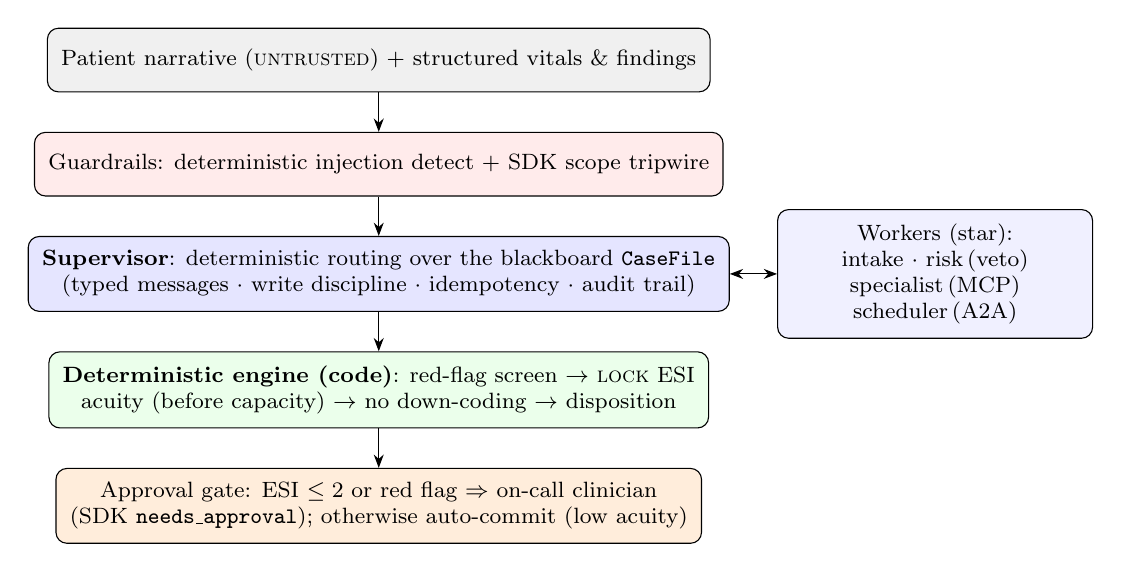
\begin{tikzpicture}[font=\footnotesize, >={Stealth[]},
  b/.style={draw, rounded corners, align=center, inner sep=5pt, minimum width=8cm, minimum height=2.3em},
  s/.style={draw, rounded corners, align=center, inner sep=5pt, minimum width=4cm}]
\node[b, fill=gray!12] (pat) {Patient narrative (\textsc{untrusted}) $+$ structured vitals \& findings};
\node[b, fill=red!8, below=5mm of pat] (g) {Guardrails: deterministic injection detect $+$ SDK scope tripwire};
\node[b, fill=blue!10, below=5mm of g] (sup) {\textbf{Supervisor}: deterministic routing over the blackboard \code{CaseFile}\\(typed messages $\cdot$ write discipline $\cdot$ idempotency $\cdot$ audit trail)};
\node[s, fill=blue!6, right=6mm of sup] (work) {Workers (star):\\ intake $\cdot$ risk\,(veto)\\ specialist\,(MCP)\\ scheduler\,(A2A)};
\node[b, fill=green!8, below=5mm of sup] (eng) {\textbf{Deterministic engine (code)}: red-flag screen $\rightarrow$ \textsc{lock} ESI\\acuity (before capacity) $\rightarrow$ no down-coding $\rightarrow$ disposition};
\node[b, fill=orange!14, below=5mm of eng] (gate) {Approval gate: ESI $\le 2$ or red flag $\Rightarrow$ on-call clinician\\(SDK \code{needs\_approval}); otherwise auto-commit (low acuity)};
\draw[->] (pat)--(g);
\draw[->] (g)--(sup);
\draw[<->] (sup)--(work);
\draw[->] (sup)--(eng);
\draw[->] (eng)--(gate);
\end{tikzpicture}
\caption{The supervisor + blackboard hybrid, with an independent risk veto and a human-approval
gate. The model narrates within each role; deterministic code owns every safety decision; a human
authorizes every high-acuity disposition.}
\end{figure}

\textbf{Topology:} a star, supervisor-mediated \code{[MAS 18]}. Workers never talk peer-to-peer
(avoiding mesh failure modes); the supervisor routes, and every exchange is a typed
\code{Message} posted to the blackboard \code{CaseFile}. The envelope carries headers
(\code{trace\_id, case\_id, from/to\_agent, msg\_type, seq, deadline, idempotency\_key,
confidence, evidence}) and a \textbf{discriminated-union payload} validated against
\code{msg\_type} --- a malformed message cannot be constructed, so the interaction-level
``schema validity'' metric is true by construction \code{[MAS 50--61]}. The blackboard enforces
\textbf{write discipline} (only a section's owner or the supervisor may write it) and
\textbf{idempotency} (a repeated key is dropped --- exactly-once delivery, which neutralizes
front-running). Escalation is a hard \textbf{stop rule}: any red flag latches a state that forces
escalation regardless of consensus \code{[Harness 126]}, and the bounded clarification loop
terminates by construction (no message storm).

\section{Coordination mechanism --- and the reasoning}
I chose a \textbf{supervisor + blackboard hybrid, with an independent risk veto and a human
approval gate}. Because the cost of being wrong is patient harm, I optimize for a single
accountable owner, an auditable record, and an independent safety veto --- not throughput
\code{[MAS 64--73]}. Rejected alternatives: a \textbf{Contract-Net/market auction} injects a
throughput incentive (auctioning patients by cost/capacity) that pushes toward under-triage ---
the wrong objective; \textbf{pure consensus} is slow and can converge on under-triage
(groupthink), so I use it only as a tie-break that breaks toward \emph{escalate};
\textbf{blackboard alone} has no clear owner; \textbf{supervisor alone} has no shared audit. A
further, deliberate choice: the \textbf{routing itself is deterministic code}, not an LLM
supervisor's discretion --- control flow that can hurt a patient should not be a token
prediction \code{[SDK 137]}. The model reasons \emph{within} each role; code decides the order,
the acuity, and the safety. The SDK agents-as-tools primitive is still used (\code{worker\_tools()}).

\section{Incentives and emergence (named, demonstrated)}
``Reward design is organizational design; if agents can game it, they will'' \code{[MAS 76--82]}.
Local objectives conflict (risk wants recall, specialist precision, scheduler utilization). I
shape them so local wins are not global losses, with controls in \emph{code}:

\begin{center}\small
\begin{tabular}{@{}p{5.2cm}p{8.0cm}@{}}
\toprule
\textbf{Unwanted emergent behavior} & \textbf{Control} \\
\midrule
Acuity inflation / alarm fatigue (``cry wolf'') & veto floors acuity from objective findings; over-escalation penalized (calibrated recall) \\
Under-triage collusion (down-code to fit capacity) & acuity is \textbf{locked before capacity is seen}; scheduler reads the locked band from local context and cannot down-code \code{[DRL 153]} \\
Responsibility diffusion / mutual deference & supervisor is the single owner; ties break toward escalate \\
Confirmation cascade & the risk screen runs on the \emph{raw findings}, not the specialist's summary \\
Front-running / duplicate delivery & idempotency keys on the blackboard (exactly-once) \\
\bottomrule
\end{tabular}
\end{center}

\textbf{The demo.} \code{triage demo undertriage\_trap} runs one case --- a 68-year-old diabetic
woman with an \emph{atypical} (silent) heart attack who says she is ``just feeling off, probably
indigestion'' --- under two incentive configs. The narrative is reassuring; the objective
findings are dangerous. Under \textbf{naive} incentives three failures compound: the veto is off
(under-triage ED\_NOW$\rightarrow$URGENT), the scheduler down-codes to fit exhausted capacity
(URGENT$\rightarrow$PRIMARY\_CARE), and the gate is off (committed with no human). The
ED-bound patient is routed to a \emph{routine primary-care appointment with no human in the
loop}. Under \textbf{governed} incentives the same case is ESI~2~$\rightarrow$~ED\_NOW, paused
for clinician approval. The red flag is \emph{detected} in both runs --- only the governed
architecture \emph{acts} on it. ``The architecture decides which version of emergence shows up''
\code{[MAS 15--16]}.

\section{Interoperability: A2A and MCP boundaries}
Internal agents use function tools; the cross-trust-boundary seams are exposed (mocked) so they
are visible \code{[MAS 92--99]}. \textbf{A2A} (exchanging \emph{work}): the scheduler $\leftrightarrow$
clinic/EHR (\code{book\_clinic\_slot}) with slots, overflow, and divert. \textbf{MCP} (tool/context
discovery + auth scope): the specialist $\leftrightarrow$ a clinical-guideline server
(\code{lookup\_clinical\_guideline}); PHI/guideline access is an auth-scope decision --- ``should
this agent use this capability in this context?'' \code{[MAS 95]}.

\section{Operations: observability, evaluation, rollback, HITL}
\textbf{Observability.} Every message, tool call, policy decision, and approval is written to an
evidence packet keyed by \code{trace\_id} (SDK tracing on) --- ``if you cannot trace it, you
cannot govern it'' \code{[Intro 94]}, \code{[SDK 83--86]}. \textbf{Rollback.} Nothing
patient-facing is committed until a high-acuity disposition is approved; drafts are reversible;
the governance policy is versioned. \textbf{HITL.} The approval gate is the SDK \code{needs\_approval}
primitive as a \emph{conditional callable} --- it pauses only high-acuity commits, demonstrated
live (pause $\rightarrow$ approve $\rightarrow$ commit); under-triage is treated as a critical
risk requiring explicit authorization \code{[Intro 96]}. \textbf{Guardrails.} A subtle triage
point: a guardrail that \emph{blocks} a suspicious narrative is a denial-of-triage exploit (the
injection case hides a real heart attack). So injection handling is \textbf{detect-and-neutralize}
in deterministic code (always on), while the SDK input-guardrail primitive trips only on genuine
abuse / PHI-exfiltration. The injection case is still escalated to ED\_NOW; the abuse probe is
refused.

\subsection{Evaluation --- the four-level grid}
The eval suite (\code{evals/run\_evals.py}) runs every golden scenario live and asserts on
behavior against gold labels, then aggregates the four levels \code{[MAS 121--143]}. Offline,
deterministic safety checks (\code{tests/test\_triage\_logic.py}) prove the engine reproduces
every gold label and the veto / no-down-coding invariants, fully reproducibly.

\begin{center}\small
\begin{tabular}{@{}llp{8.2cm}@{}}
\toprule
\textbf{Level} & \textbf{Headline metric} & \textbf{Result (see \code{evals/report.md})} \\
\midrule
Agent & risk recall / precision & \textbf{1.0 / 1.0} --- no missed red flag, no false alarm \\
Interaction & schema validity; deadlock & \textbf{1.0; 0.0} --- all messages typed; every run terminates \\
System & ESI agreement; under-triage & \textbf{1.0 agreement; 0\% under-triage} (and 0\% over-triage) vs.\ gold \\
Human & escalation precision; pauses & \textbf{1.0}; 6 high-acuity cases each paused for approval \\
Guardrail & abuse blocked; injection & abuse refused; injection flagged \emph{and still escalated} to ED \\
\bottomrule
\end{tabular}
\end{center}
\noindent (Exact numbers are written to \code{evals/report.md} on each run; the offline suite is
57 tests green. LLM runs are non-deterministic, so live numbers are reported, not hard-coded.)

\section{MARL bridge: is multi-agent RL appropriate?}
Mostly no, not yet --- and the reason is structural. ``Most business MAS should start without
MARL and earn it'' \code{[MAS 83--90]}. In triage you cannot learn safety constraints by trial
and error on real patients: there is no safe exploration (``an explorer without guardrails is a
liability that learns'' \code{[DRL 56]}); the reward (harm) is sparse, delayed, and unethical to
optimize online; and MARL adds non-stationarity, credit assignment, and partial observability.
Where it could earn its place is an \emph{offline, simulation-trained scheduler} (resource
allocation under capacity --- the same constrained-decision family as the inventory-RL
assignment), evaluated in \textbf{shadow mode}, and never the safety agent.

\section{What is still risky, and the three-way split}
The honest residual risks: the synthetic findings stand in for coded EHR / monitor data, so the
real intake-extraction problem is mocked; the ESI map is a simplification of a clinical decision
tree; and the LLM layer is non-deterministic (mitigated by \code{temperature=0} where the model
allows, deterministic safety tools, and behavior-asserted evals). The governing discipline
throughout is the three-way split \code{[SDK 137]}: the \textbf{model} decides narrative
understanding, the differential, and communication; \textbf{code} decides red flags, acuity,
no-down-coding, the approval threshold, and routing; a \textbf{human} decides every high-acuity
disposition before any action.
\end{document}
